\section{Visualisation du corpus dans PixPlot}

\begin{figure}[H]
    \centering
    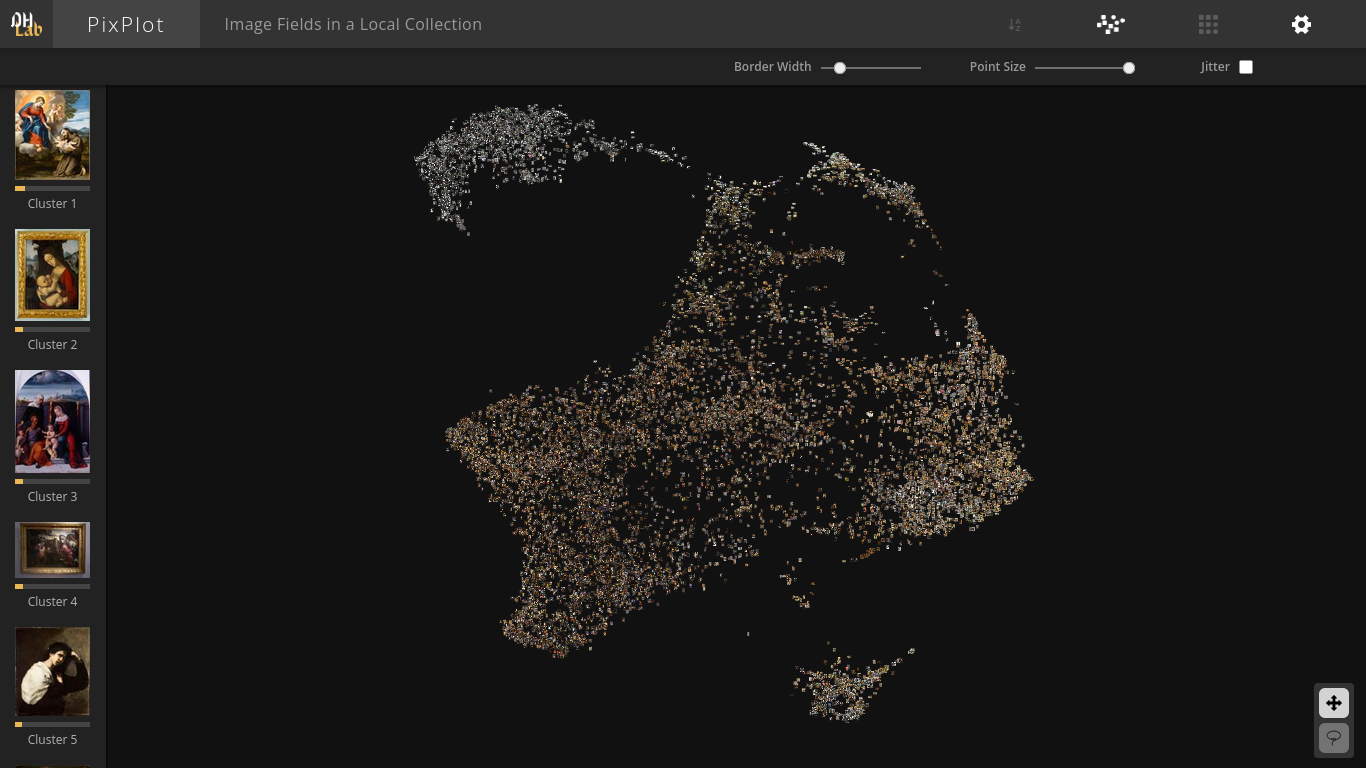
\includegraphics[width=1\textwidth]{annexes/figures/PP-generale.png}
    \caption{Visualisation générale des tableaux du RETIF dans PixPlot.}
    \label{fig:PP-general}
\end{figure}

\begin{figure}[H]
    \centering
    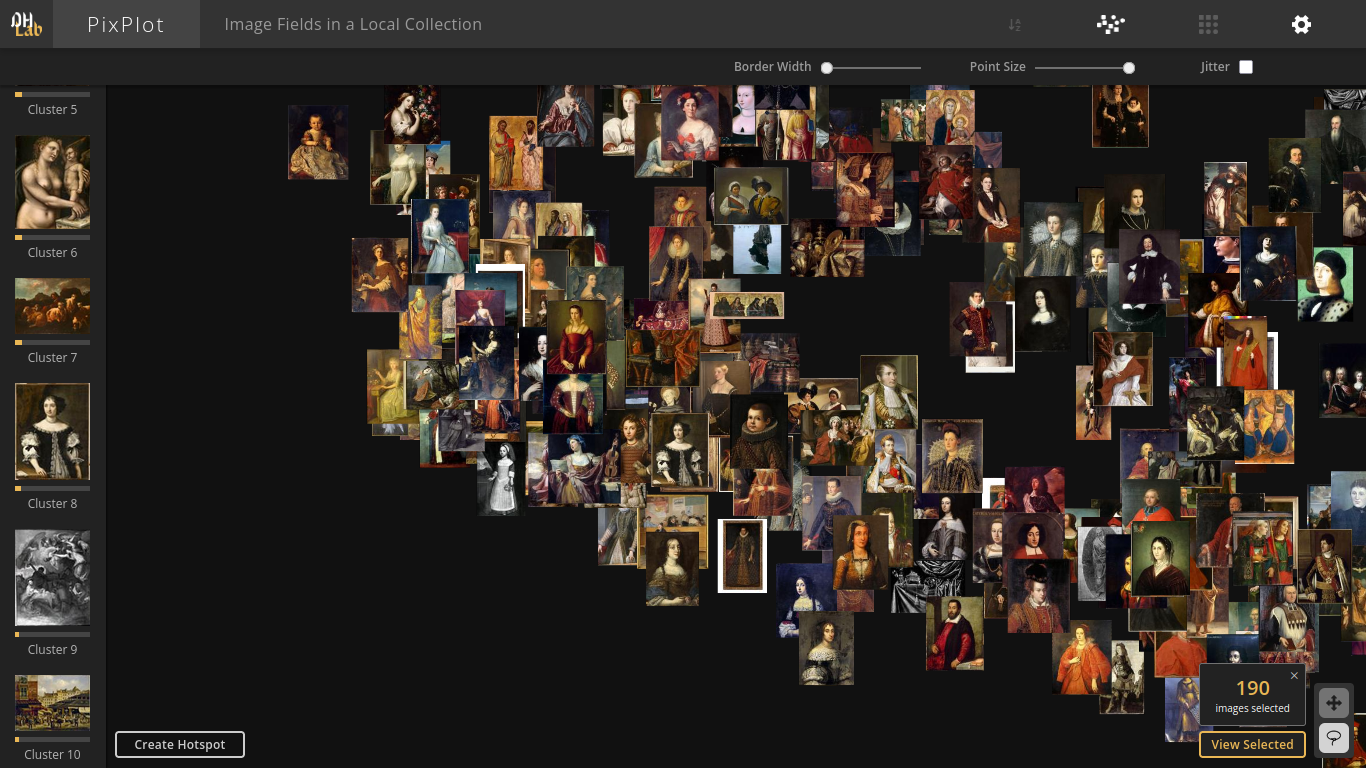
\includegraphics[width=1\textwidth]{annexes/figures/PP-portraits.png}
    \caption{Cluster de portraits identifié dans l'angle inférieur gauche de la visualisation du RETIF dans PixPlot.}
    \label{fig:PP-portraits}
\end{figure}

\begin{figure}[H]
    \centering
    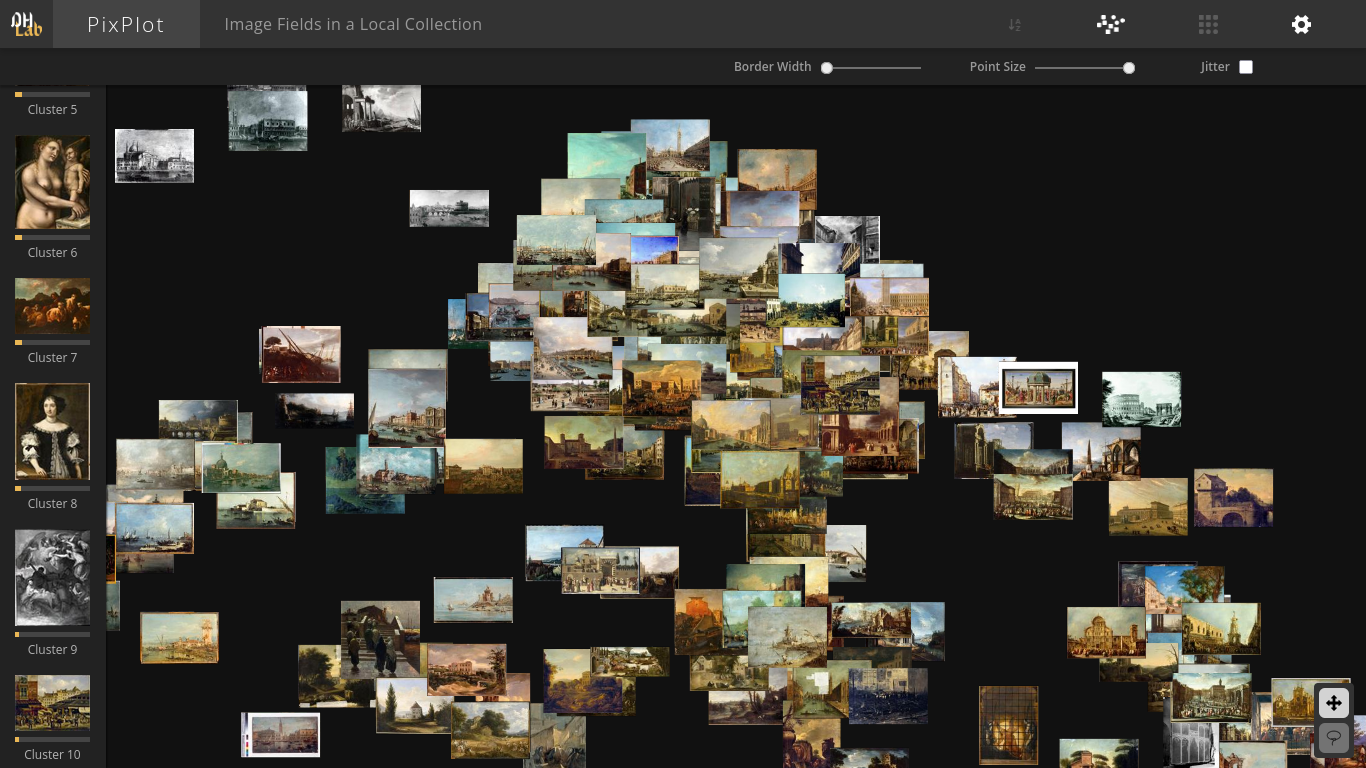
\includegraphics[width=1\textwidth]{annexes/figures/PP-vedute.png}
    \caption{Cluster de paysages urbains dans l'angle supérieur droit de la visualisation du RETIF dans PixPlot.}
    \label{fig:PP-vedute}
\end{figure}

\begin{figure}[H]
    \centering
    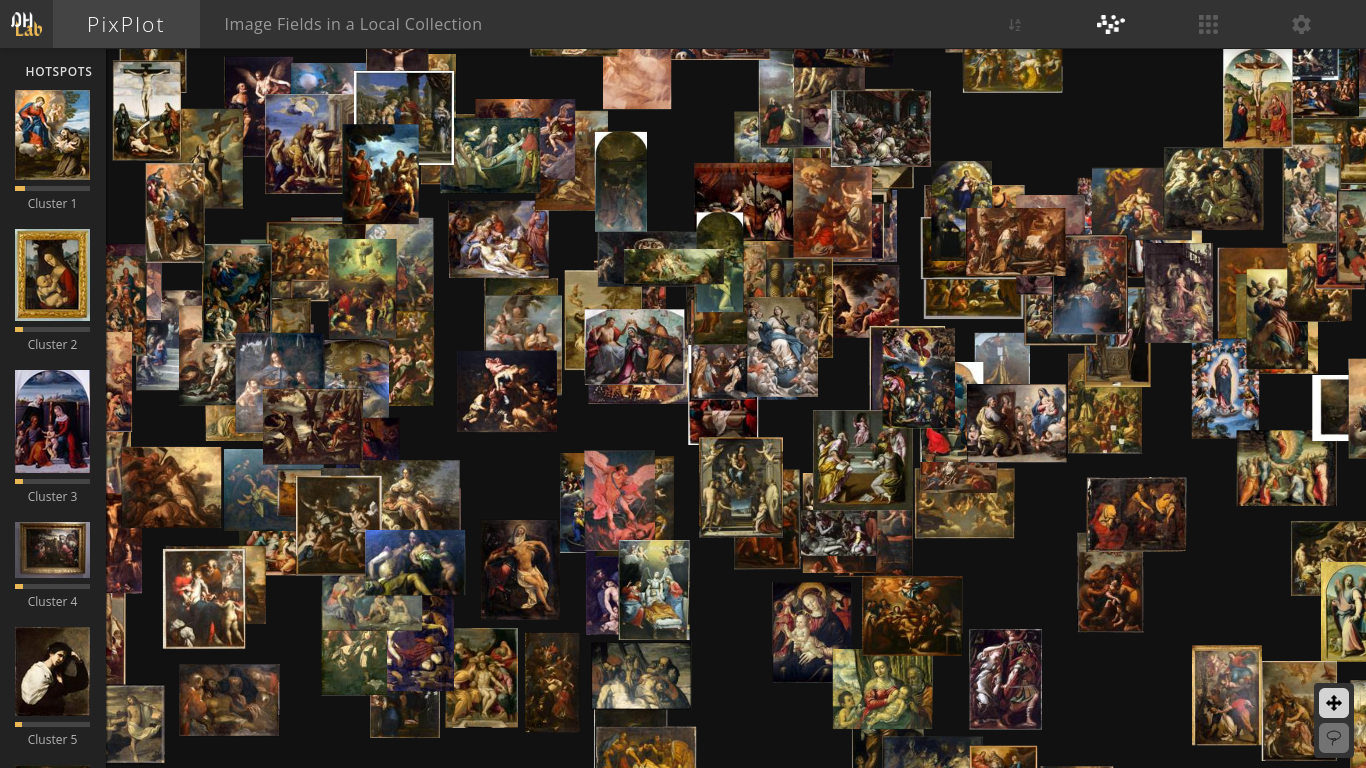
\includegraphics[width=1\textwidth]{annexes/figures/PP-scenes.png}
    \caption{Cluster des scènes religieuses et mythologiques au centre de la visualisation du RETIF dans PixPlot.}
    \label{fig:PP-scenes}
\end{figure}

\begin{figure}[H]
    \centering
    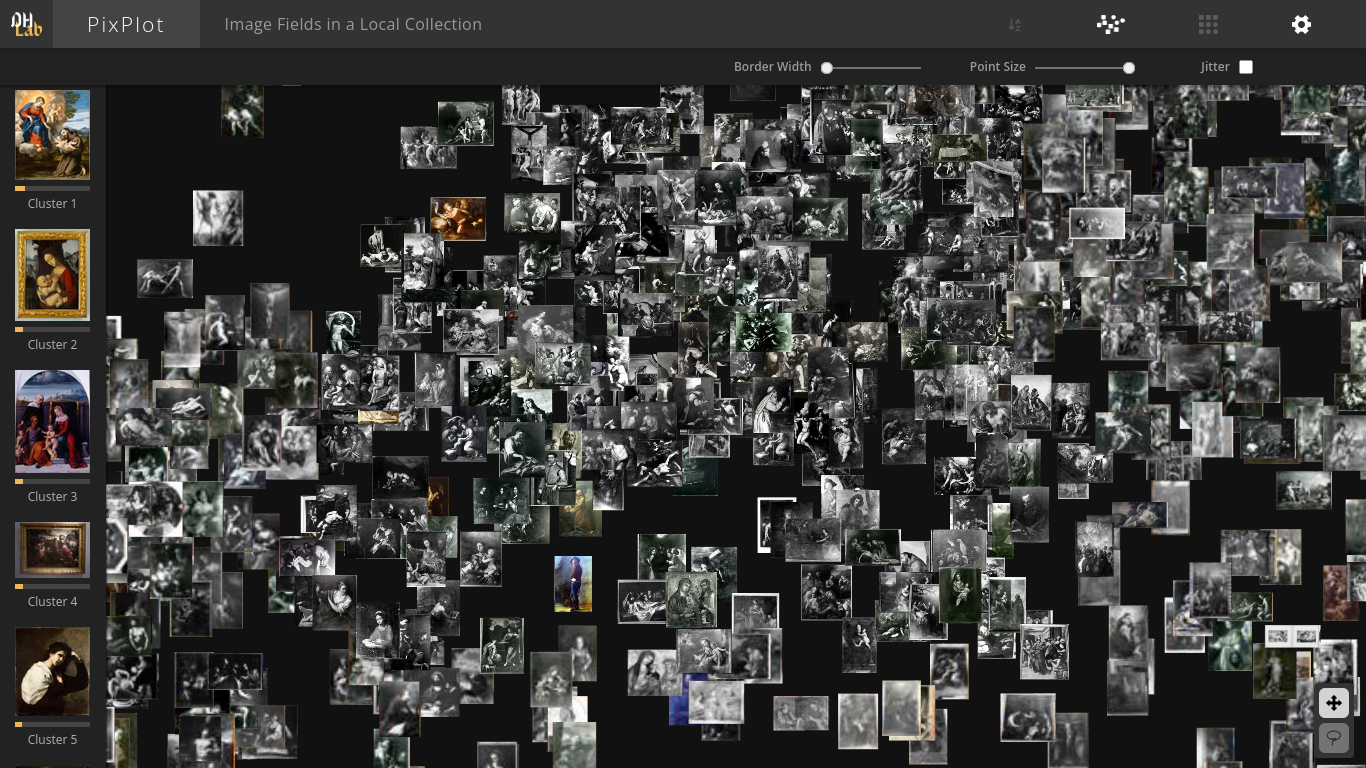
\includegraphics[width=1\textwidth]{annexes/figures/PP-n&b.png}
    \caption{Cluster des photographies en noir et blanc dans l'angle supérieur gauche de la visualisation du RETIF dans PixPlot.}
    \label{fig:PP-n&b}
\end{figure}

\begin{figure}[H]
    \centering
    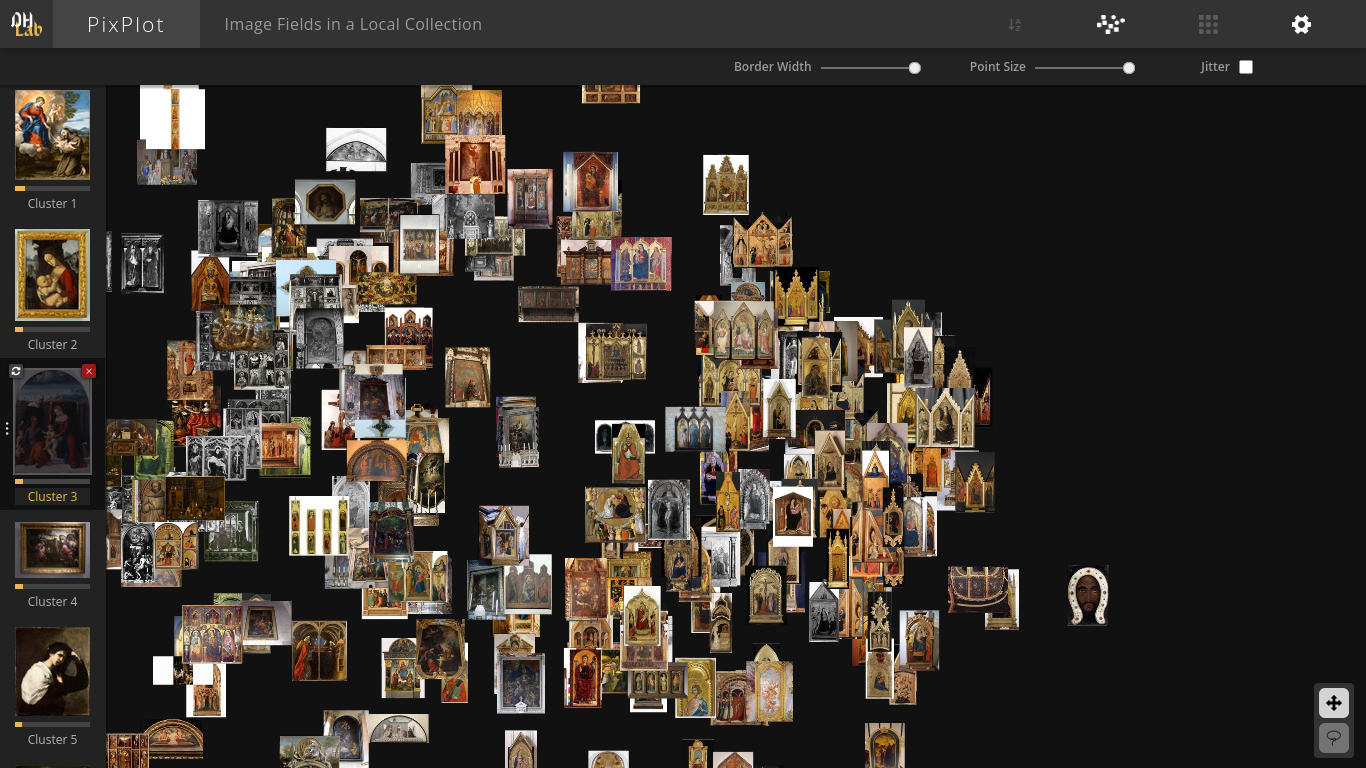
\includegraphics[width=1\textwidth]{annexes/figures/PP-polyptiques.png}
    \caption{Cluster des panneaux médiévaux et des tableaux dans leur contexte dans le bord droit  de la visualisation du RETIF dans PixPlot.}
    \label{fig:PP-polyptiques}
\end{figure}

\begin{figure}[H]
    \centering
    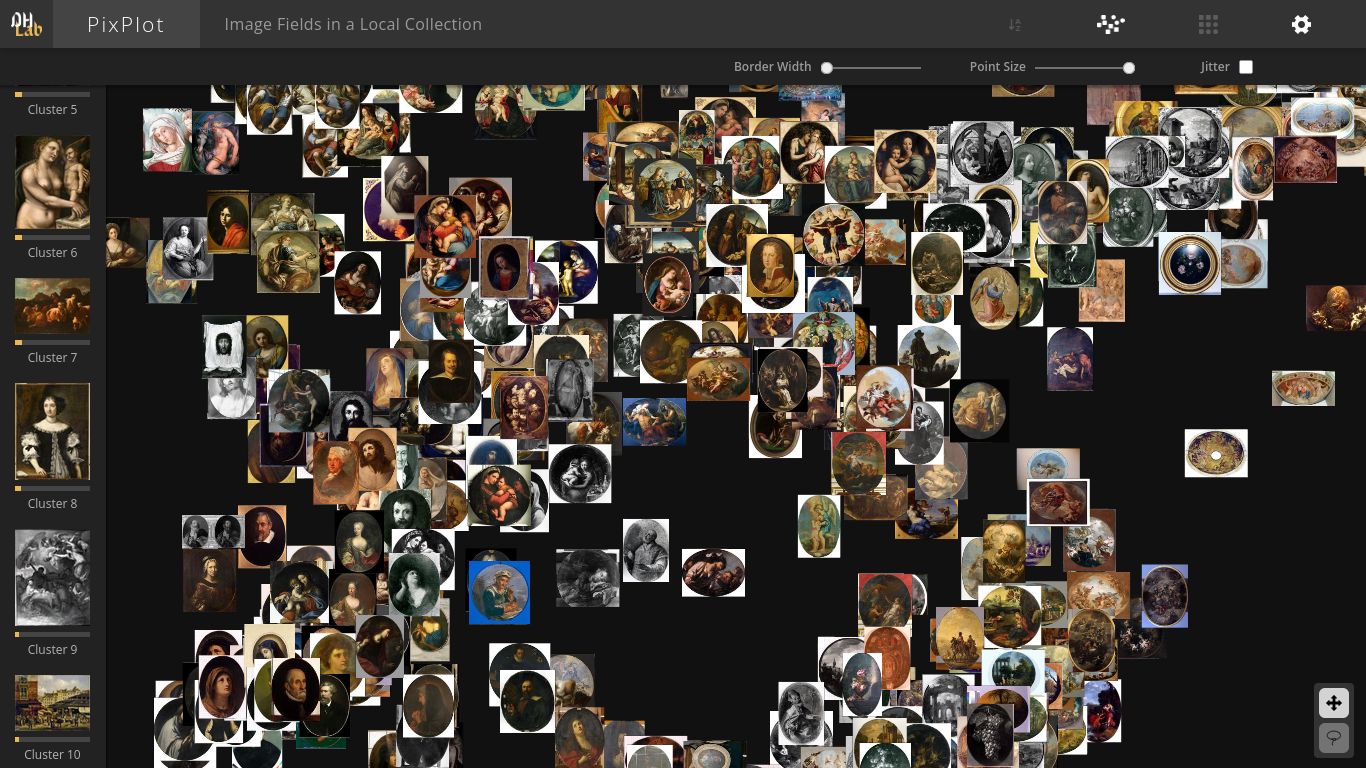
\includegraphics[width=1\textwidth]{annexes/figures/PP-ronds.png}
    \caption{Cluster des tableaux aux formats inhabituels (circulaire, ovale, hexagonal) dans l'angle inférieur droit de la visualisation du RETIF dans PixPlot.}
    \label{fig:PP-ronds}
\end{figure}

\section{Visualisation du corpus dans Panoptic}

\begin{figure}[H]
    \centering
    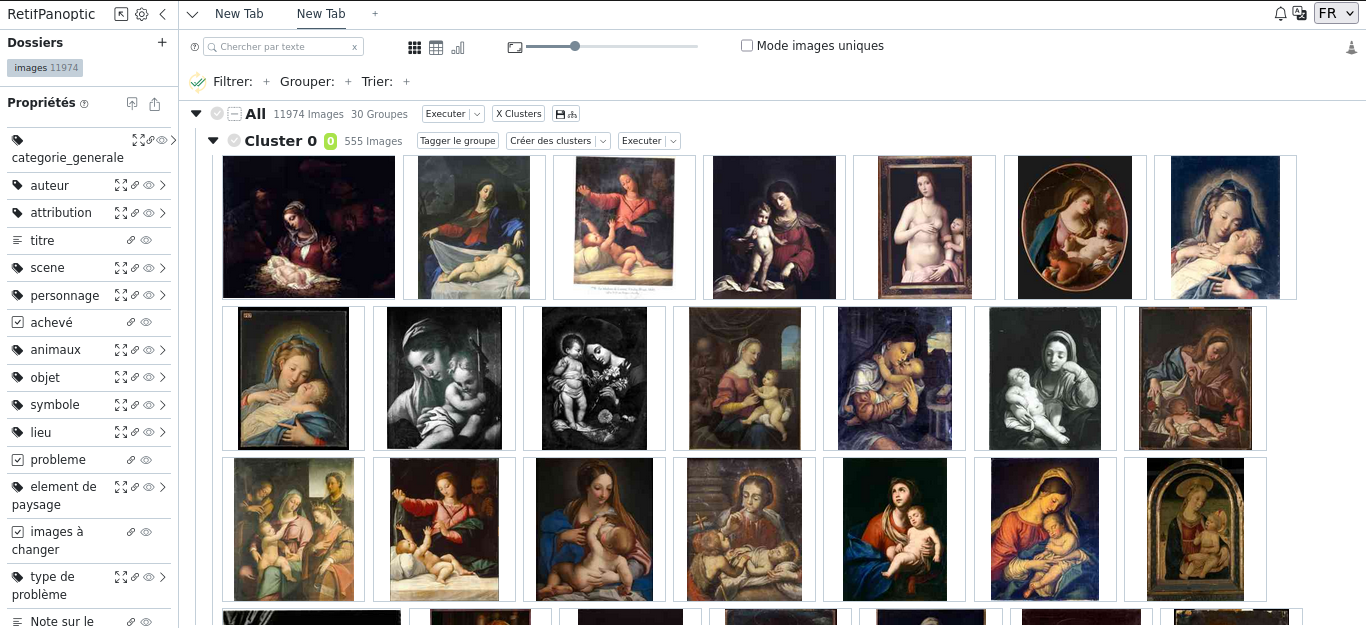
\includegraphics[width=1\textwidth]{annexes/figures/Pa-Vierges.png}
    \caption{Cluster des Vierge à l'Enfant dans Panoptic.}
    \label{fig:Pa-Vierges}
\end{figure}
